\documentclass[12pt]{article}
\usepackage{tikz}
\usepackage{bm}
\usepackage{amsmath,amssymb}
\usepackage{textcomp}
\usepackage{listings}
\usepackage[colorlinks=true,pagebackref,linkcolor=blue]{hyperref}
\textwidth=7in
\textheight=9.5in
\topmargin=-1in
\headheight=0in
\headsep=.5in
\hoffset -.85in


\lstset{
basicstyle=\footnotesize\ttfamily,
language=R,
upquote=true,
breakatwhitespace=true,
columns=fullflexible,
keepspaces,
numbers=none,
tabsize=3,
frame=b,
framextopmargin=20pt,
showstringspaces=false,
extendedchars=true
}

\pagestyle{empty}

\renewcommand{\thefootnote}{\fnsymbol{footnote}}

\usepackage{Sweave}

\begin{document}
\Sconcordance{concordance:jhuang63HW3.tex:jhuang63HW3.Rnw:%
1 34 1 1 0 88 1}

\Sconcordance{concordance:jhuang63HW3.tex:jhuang63HW3.Rnw:%
1 34 1 1 0 88 1}




\begin{center}
{\bf AMS 550.400 \qquad Homework 3 \qquad Due Date: Nov 19}\\
\vskip.2in
{\footnotesize Last Compiled on \today}
\end{center}

\setlength{\unitlength}{1in}

\begin{picture}(6,.1)
\put(0,0) {\line(1,0){6.25}}
\end{picture}

\renewcommand{\arraystretch}{2}

\noindent {\bf Solution for Ex 7.18}

\begin{itemize}
\item[(a)] Use Sweave to accomplish goal, we can get the figure: jhuang63HW3-1.png (uploaded to github file)\\
\includegraphics{jhuang63HW3-001}
\begin{lstlisting}[caption=R Codes for Ex 7.18, label=code:plot]
\includegraphics{jhuang63HW3-002}
\end{lstlisting}
\end{itemize}
\begin{itemize}
\item[(b)]
The rank of $A$ is 2 and the rank of $B$ is 1.\\
Generating the second and third colunms of $A$ from the first column will change the determinant of this matrix. So, it does not work.\\
\end{itemize}

\begin{itemize}
\item[(c)] See the following description:\\
\begin{Schunk}
\begin{Sinput}
> a = cbind(A[1:2, 3])
> A12 = A[1:2, 1:2]
> dA12 = det(A12)
> x = solve(A12, a)
\end{Sinput}
\end{Schunk}
Here is how the linear combination could create the third column from the first two:\\
For $A$:\\
$$c3=-1*c1+2*c2.$$
For $B$:\\
$$c3=x*c1+y*c2$$ for all $x$ and $y$ that satisfy $1*x+2*y=3$.\\

The determinant of the rank 2 submatrix $A12$ is $\det(A12)=\det
\begin{pmatrix}
1&2\\
2&3
\end{pmatrix}
=-1 \neq 0$,

\end{itemize}

So, this matrix can be used with corresponding coordinates in the third column to derive the linear combination.\\

For $B$, the rank is $1$, so we can use the first row of it to find the linear combination. The coefficient for the 1st column $x$ and the 2nd column $y$ can be any numbers that satisfy following demand:$$1*x+2*y=3$$\\


\paragraph{Ex 7.24}
\begin{itemize}
    \item \verb+[COMMIT]+ use \verb+lstlisting+ to list your R code
    \item \verb+[COMMIT]+ use R/Sweave for computation, but do not use the built-in \verb+dist+
        function
\begin{lstlisting}
\end{lstlisting}
    \item \verb+[COMMIT]+ use R/Sweave for computation, and this time, do use the built-in \verb+dist+
        function for comparison
\begin{lstlisting}
\end{lstlisting}
    \item \verb+[COMMIT]+ make sure to explain your computation, e.g., compare the two
        computations
\end{itemize}

\newpage
\noindent{\bf Solution for Ex 7.24}\\
\begin{lstlisting}[caption=R codes for Ex 7.24, label=code:distance]
M=A%*%t(A)
c=cbind(diag(M))
one=cbind(c(1,1,1,1))
D=c%*%t(one)+one%*%t(c)-2*M
Dis=sqrt(D)
\end{lstlisting}

\begin{itemize}
\item Without Built-in dist function:\\
\begin{Schunk}
\begin{Sinput}
> M = A %*% t(A)
> c = cbind(diag(M))
> one = cbind(c(1, 1, 1, 1))
> D = c %*% t(one) + one %*% t(c) - 2 * M
> Dis = sqrt(D)
\end{Sinput}
\end{Schunk}

\item With Built-in dist function:\\
\begin{Schunk}
\begin{Sinput}
> di = dist(M)
> distance = as.matrix
\end{Sinput}
\end{Schunk}
Now, we can calculate the distance matrix:
$$D=
\begin{pmatrix}
0&3&12&27\\
3&0&3&12\\
12&3&0&3\\
27&12&3&0
\end{pmatrix}$$
  
\end{itemize}

If there are no built-in dist functions can be used, then we shall use the formula in the book to derive a matrix $M=AA'$,then calculate the distance matrix from the diagonal entries of $X$, matrix $X$ as well as a one vector.\\

If there are built-in dist funtions can be used, we just need to use the built-in R DIST function to do the calculation directly.\\

\paragraph{Ex 7.30}
Omit (c), (d) and (e).
The necessary data is saved in \verb+matlabclown.RData+
and can be found from the course git folder.
The followings are the equivalent R version:
\begin{lstlisting}
load('matlabclown.RData')
image(X) # omit this in your Sweave code
svdX = svd(X)
U = svdX$u
S = diag(svdX$d)
V = svdX$v
k = 10
M = U[,1:k,drop=FALSE] %*% S[1:k,1:k,drop=FALSE] %*% t(V[,1:k,drop=FALSE])
image(M) # omit this in your Sweave code
image(M,col=gray.colors(k))
\end{lstlisting}
\begin{itemize}
\item[(a)] \verb+[COMMIT]+ choose a small, a medium and a large value for $k$
\begin{itemize}
\item for each $k$,
\begin{itemize}
\item do \verb+[COMMIT]+
\item your performance evaluation is to be included as a caption,
and change \verb+tinyK+, \verb+width+ and \verb+height+ accordingly
\begin{lstlisting}
\begin{figure}
\centering
\begin{Schunk}
\begin{Sinput}
> tinyK = 1
\end{Sinput}
\end{Schunk}
\includegraphics{jhuang63HW3-009}
\caption{<YOUR PERFORMANCE EVALUATION> on $1$}
\label{fig:matlabclownKaNumber}
\end{figure}
\end{lstlisting}
\end{itemize}
\end{itemize}
\item[(b)]
\begin{itemize}
\item \verb+[COMMIT]+ code up all your computation using R/Sweave
before starting to type your explanation
\begin{lstlisting}
\end{lstlisting}
\item \verb+[COMMIT]+ write your explanation referring to the
numbers computed in the previous step, using
\verb++
\end{itemize}
\end{itemize}

\newpage
\noindent{\bf Solution for Ex 7.30:}
\begin{itemize}
    \item[(a)] 
\begin{figure}
    \centering
\begin{Schunk}
\begin{Sinput}
> tinyK = 1
> smallK = 20
> mediumK = 80
> largeK = 150
> load("/Users/hj//550400/jhuang63HW3.git/matlabclown.RData")
> svdX = svd(X)
> U = svdX$u
> S = diag(svdX$d)
> V = svdX$v
> k = tinyK
> M = U[, 1:k, drop = FALSE] %*% S[1:k, 1:k, drop = FALSE] %*% 
+     t(V[, 1:k, drop = FALSE])
> image(M, col = gray.colors(k))
\end{Sinput}
\end{Schunk}
\includegraphics{jhuang63HW3-011}
\caption{The Poorest Performance on $1$}
    \label{fig:matlabclownK1}
\end{figure}
\begin{figure}
    \centering
\begin{Schunk}
\begin{Sinput}
> tinyK = 1
> smallK = 20
> mediumK = 80
> largeK = 150
> load("/Users/hj//550400/jhuang63HW3.git/matlabclown.RData")
> svdX = svd(X)
> U = svdX$u
> S = diag(svdX$d)
> V = svdX$v
> k = smallK
> M = U[, 1:k, drop = FALSE] %*% S[1:k, 1:k, drop = FALSE] %*% 
+     t(V[, 1:k, drop = FALSE])
> image(M, col = gray.colors(k))
\end{Sinput}
\end{Schunk}
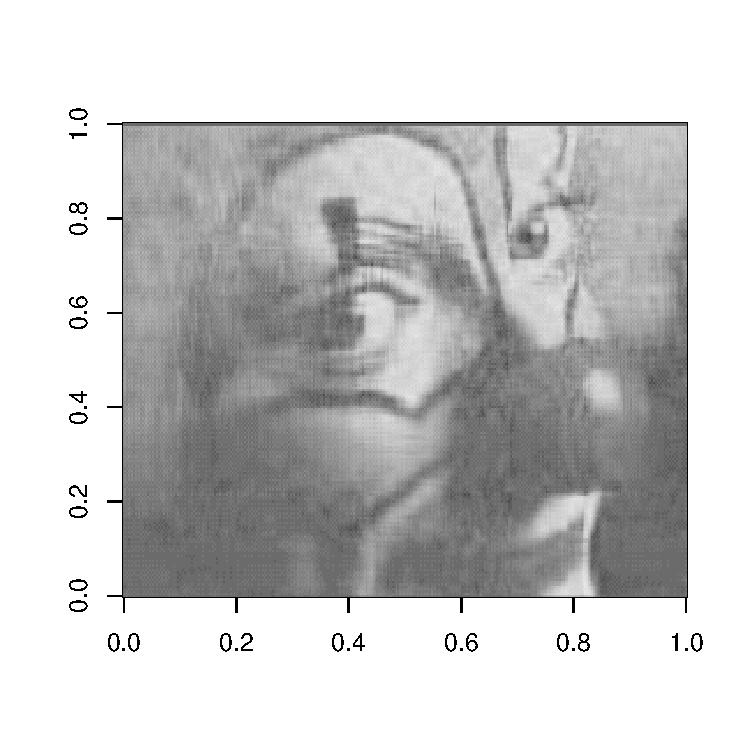
\includegraphics{jhuang63HW3-012}
\caption{Poor Performance on $20$}
    \label{fig:matlabclownK10}
\end{figure}
\begin{figure}
    \centering
\begin{Schunk}
\begin{Sinput}
> tinyK = 1
> smallK = 20
> mediumK = 80
> largeK = 150
> load("/Users/hj//550400/jhuang63HW3.git/matlabclown.RData")
> svdX = svd(X)
> U = svdX$u
> S = diag(svdX$d)
> V = svdX$v
> k = mediumK
> M = U[, 1:k, drop = FALSE] %*% S[1:k, 1:k, drop = FALSE] %*% 
+     t(V[, 1:k, drop = FALSE])
> image(M, col = gray.colors(k))
\end{Sinput}
\end{Schunk}
\includegraphics{jhuang63HW3-013}
\caption{Good Performance on $80$}
    \label{fig:matlabclownK75}
\end{figure}
\begin{figure}
    \centering
\begin{Schunk}
\begin{Sinput}
> tinyK = 1
> smallK = 20
> mediumK = 80
> largeK = 150
> load("/Users/hj//550400/jhuang63HW3.git/matlabclown.RData")
> svdX = svd(X)
> U = svdX$u
> S = diag(svdX$d)
> V = svdX$v
> k = largeK
> M = U[, 1:k, drop = FALSE] %*% S[1:k, 1:k, drop = FALSE] %*% 
+     t(V[, 1:k, drop = FALSE])
> image(M, col = gray.colors(k))
\end{Sinput}
\end{Schunk}
\includegraphics{jhuang63HW3-014}
\caption{Better Performance on $150$}
    \label{fig:matlabclownK150}
\end{figure}

\item[(b)]

\item[(c)]
Based on the four figures we have now, it is obvious that clown pictures become clearer as the value of K increasing from small to big. And the corresponding rate are 0.204574122478363,0.57410568828537,0.834591398235888,0.964020698568418 respectively.
\end{itemize}

\vskip0.25in
\begin{center}
\textbf{Problems from Chapter 4: Multidimensional Scaling}
\end{center}

\newpage
\noindent {\bf Solution for Ex 4.1:}\\
\begin{figure}[h!]
    \centering
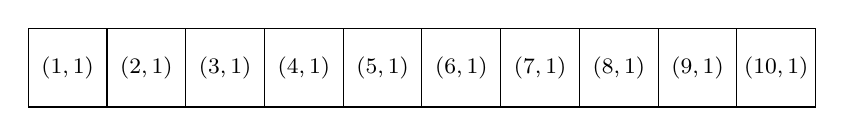
\begin{tikzpicture}
  \foreach \x in {1,2,...,10}
    \foreach \y in {1}
    {
      \draw (\x,\y) +(-.5,-.5) rectangle ++(.5,.5);
      \draw (\x,\y) node{\footnotesize $(\x,\y)$};
    }
\end{tikzpicture}
\caption{first ten objects on a Line}
\label{fig:tenobjects}
\end{figure}
\begin{lstlisting}[caption=R codes, label={code:}]

M=matrix(rep(1,51*51),nrow=51,byrow=TRUE)
for (i in 1:51){
  for (j in 1:51){
    if(i == j) M[i,j]=9
    else if(abs(i-j)>=22 & abs(i-j)<=24) M[i,j]=1
    else if(abs(i-j)>=19 & abs(i-j)<=21) M[i,j]=2
    else if(abs(i-j)>=16 & abs(i-j)<=18) M[i,j]=3
    else if(abs(i-j)>=13 & abs(i-j)<=15) M[i,j]=4
    else if(abs(i-j)>=10 & abs(i-j)<=12) M[i,j]=5
    else if(abs(i-j)>=7 & abs(i-j)<=9) M[i,j]=6
    else if(abs(i-j)>=4 & abs(i-j)<=6) M[i,j]=7
    else if(abs(i-j)>=1 & abs(i-j)<=3) M[i,j]=8
    else M[i,j]=0
  }
}
D=matrix(rep(1,51*51),nrow=51,byrow=TRUE)
for (i in 1:51){
  for (j in 1:51){
  D[i,j]=sqrt(M[i,i]+M[j,j]-2*M[i,j])
  }
}
X_cmd=cmdscale(D)
plot(X_cmd,col=heat.colors(51),pch=10)
\end{lstlisting}

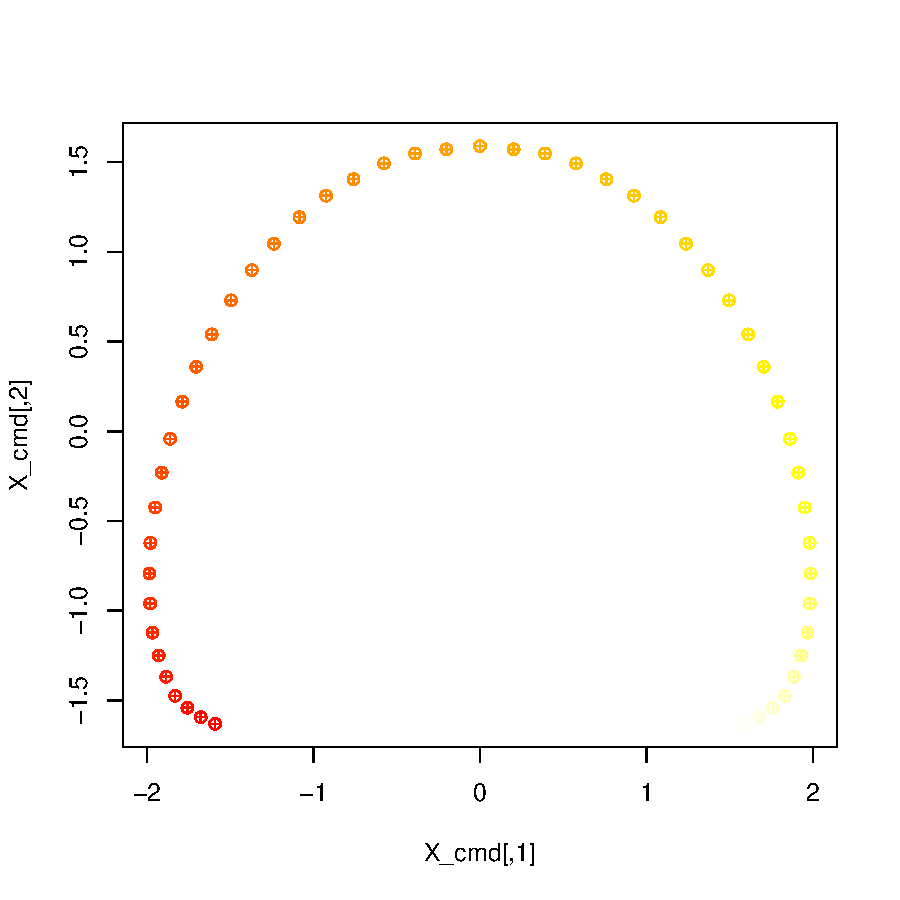
\includegraphics{jhuang63HW3-016}
\newline
From the graphic above, every point is similar to its neighbors while the similarity dies down with distance. The disimilarity in colar represents the disimilarity of each point.
\\

\paragraph{Ex 4.3}
\begin{itemize}
\item \verb+[COMMIT]+ list your R code using \verb+lstlisting+
\item \verb+[COMMIT]+ load the data
(\verb+require(MVA);data(gardenflowers)+) and compute using R/Sweave
\item \verb+[COMMIT]+ include a plot of (relative) positions using R/Sweave
\item \verb+[COMMIT]+ allocate at least a quarter page of \emph{text} explaining the result
\end{itemize}

\noindent {\bf Solution for Ex 4.3:}\\
\begin{lstlisting}[caption=R codes for Flowers Comparison, label={code:gardenflowers}]
require(MVA)
data(gardenflowers)
flowers_m=cmdscale(gardenflowers,k=17,eig=TRUE)
x=flowers_m$points[,1]
y=flowers_m$points[,2]
plot(x,y,xlab = "First column of input", ylab = "Second column of input",xlim = range(x)*1.5, type = "n")
text(x, y, labels = colnames(as.matrix(gardenflowers)), cex = 0.5)
\end{lstlisting}

\includegraphics{jhuang63HW3-017}

\bibliographystyle{plain}
\nocite{*}
\bibliography{biblio}

\end{document}
